\begin{figure}[htbp]
    \centering
    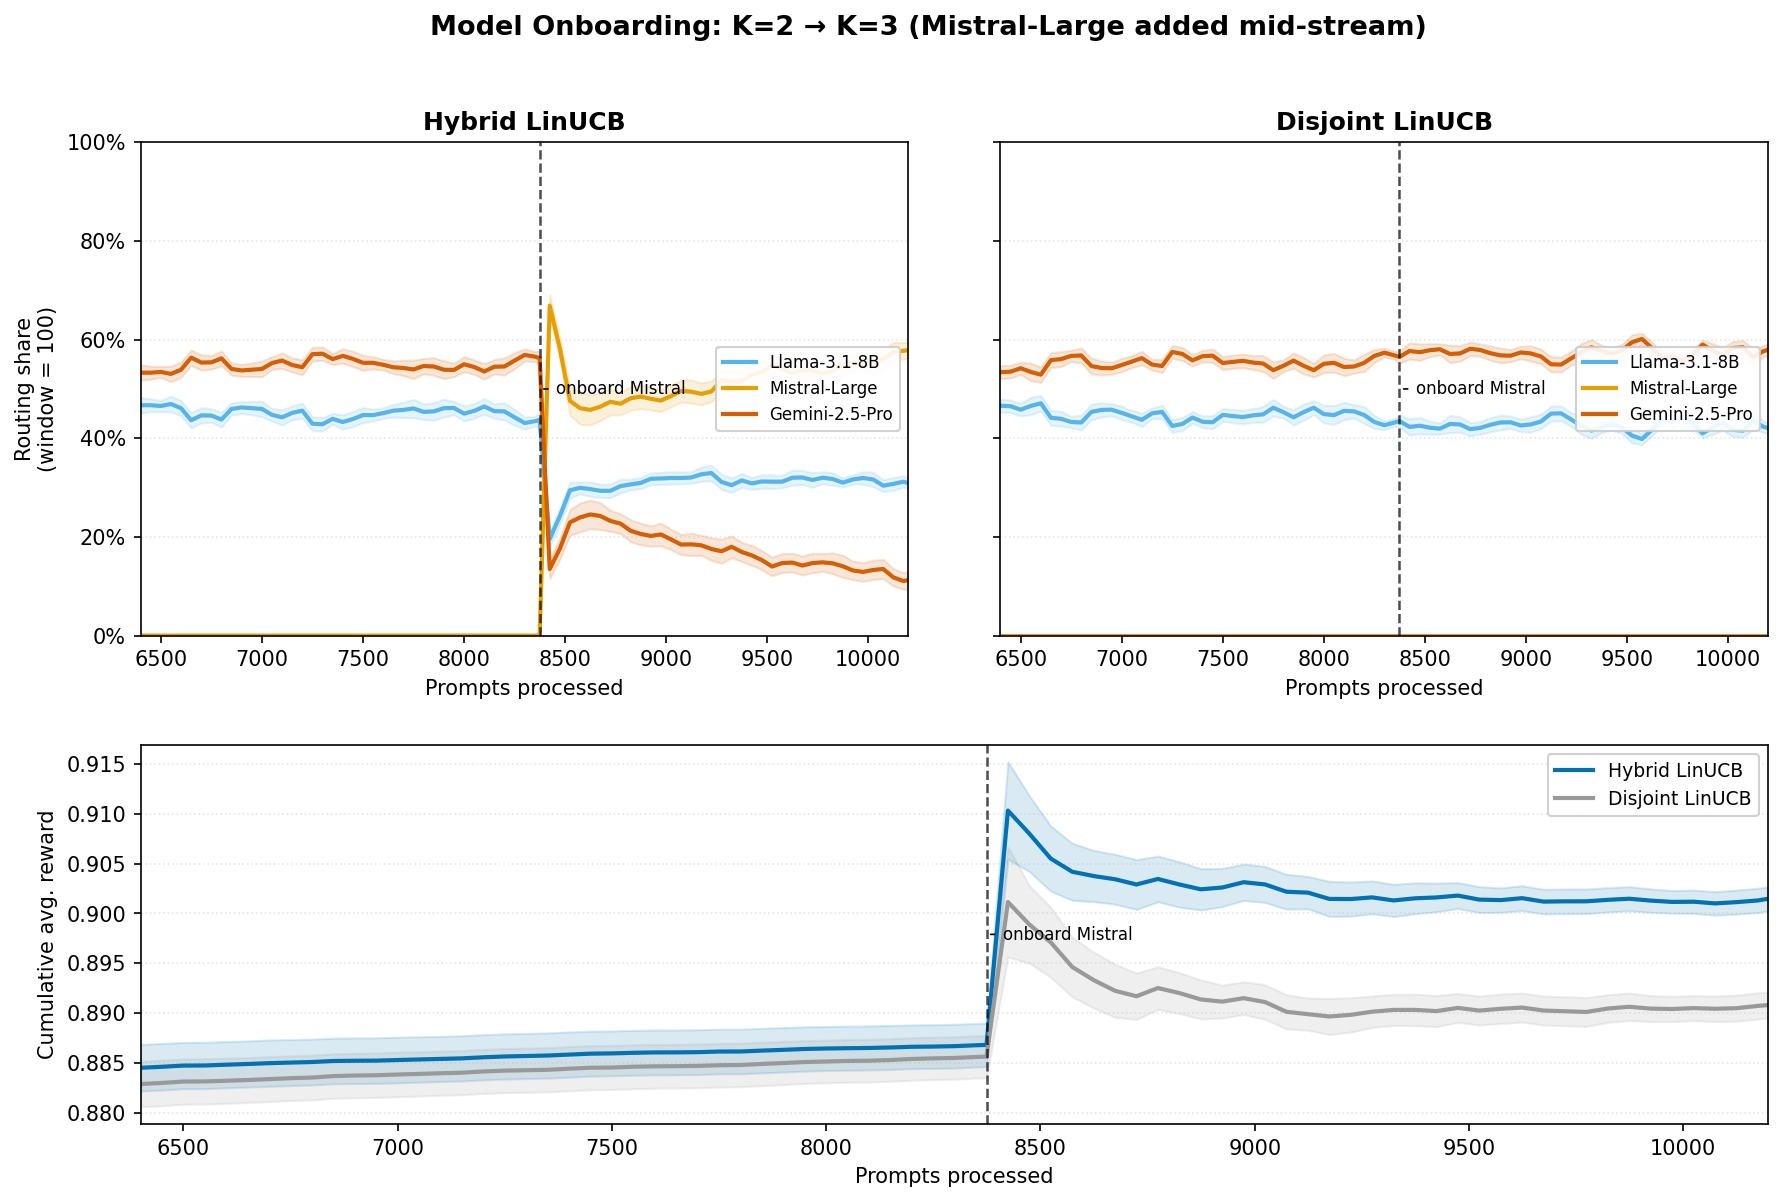
\includegraphics[width=\linewidth]{../experiments/03_figure/results/figure3_onboarding.pdf}
    \caption{Model onboarding: adding Mistral-Large-2512 to a $K{=}2$
    portfolio (Llama-3.1-8B + Gemini-2.5-Pro).
    All panels show windowed routing share (last 100 prompts).
    %
    \textbf{Left (Hybrid LinUCB):}\ the shared $\beta$ from $K{=}2$
    training transfers to the newcomer.  Mistral's share rises rapidly
    and Gemini's collapses as the router discovers that Mistral delivers
    ${\sim}99\%$ of Gemini's quality at $1/29$th the cost.
    %
    \textbf{Centre (Disjoint LinUCB, ablation):}\ without cross-arm
    parameter sharing, the newcomer must learn its quality profile from
    scratch, resulting in slower adoption.
    %
    \textbf{Right (overlay):}\ Mistral's windowed share for both
    conditions on the same axes.  Dotted lines and markers indicate
    the convergence point (share within $\pm 5$pp of final value).
    Both policies converge to the same steady-state routing mix,
    confirming that the shared $\beta$ is a \emph{speed} advantage,
    not a fundamental one.
    %
    Both conditions share identical $K{=}2$ warmup priors and
    Corralling configuration; only the shared $\beta$ differs.
    Setup: $\lambda{=}0.20$ (median from the K{=}2 Pareto sweep),
    $n{=}8{,}374$ training prompts (K=2), $n{=}1{,}824$ test prompts
    (K=3), averaged over 3~seeds.
    Hyperparameters ($\alpha{=}0.05$, $\neff{=}50$, Corralling)
    from val-tuned corralling config.
    }
    \label{fig:onboarding_k3}
\end{figure}
